% Totoro sitting in the snow
% By Noa Hoffmann and Pascal Günthner, 21.12.2020
\documentclass[tikz,11pt]{{standalone}}
\usepackage{calligra}
\usepackage[T1]{fontenc}
\usetikzlibrary{positioning, chains, calc, fit, arrows.meta, shapes}

\begin{document}    
        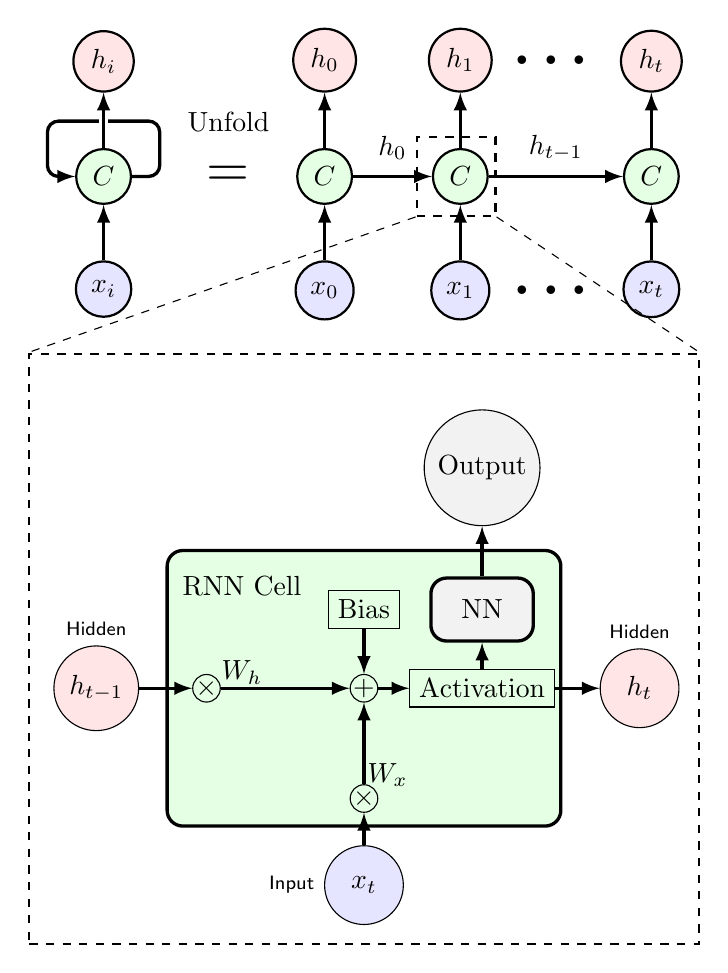
\begin{tikzpicture}[
        item/.style={circle,draw,thick},
        itemc/.style={item,on chain,join},             
        cell/.style={% For the main box
            rectangle, 
            rounded corners=2mm, 
            draw,
            very thick,
            fill=green!10,
            },
        operator/.style={%For operators like +  and  x
            circle,
            draw,
            inner sep=-0.5pt,
            minimum height =.35cm,
            },
        function/.style={%For functions
            ellipse,
            draw,
            inner sep=1pt
            },
        ct/.style={% For external inputs and outputs
            circle,
            draw,
            minimum height =1.cm,
            },
        gt/.style={% For internal inputs
            rectangle,
            draw
            },
        mylabel/.style={% something new that I have learned
            font=\scriptsize\sffamily
            },
        ArrowC1/.style={% Arrows with rounded corners
            rounded corners=.25cm,
            thick,
            },
        ArrowC2/.style={% Arrows with big rounded corners
            rounded corners=.5cm,
            thick,
            },
            ]
         \begin{scope}[start chain=going right,nodes=itemc,every
         join/.style={-latex,very thick},local bounding box=chain]
         \path node [fill=green!10] (W0) {$C$} node [fill=green!10] (W1)  {$C$} node[xshift=2em, fill=green!10] (Wt)
         {$C$};
         \end{scope}
         \node[left=1em of chain,scale=2] (eq) {$=$};
         \node[left=2em of eq,item,fill=green!10] (WL) {$C$};
         \path (WL.west) ++ (-1em,2em) coordinate (aux);
         \draw[very thick,-latex,rounded corners] (WL.east) -| ++ (1em,2em) -- (aux) 
         |- (WL.west);
         \foreach \X in {0,1,t} 
         {\draw[very thick,-latex] (W\X.north) -- ++ (0,2em)
         node[above,item,fill=red!10] (h\X) {$h_\X$};
         \draw[very thick,latex-] (W\X.south) -- ++ (0,-2em)
         node[below,item,fill=blue!10] (x\X) {$x_\X$};}
         \draw[white,line width=0.8ex] (WL.north) -- ++ (0,1.9em);
         \draw[very thick,-latex] (WL.north) -- ++ (0,2em)
         node[above,item,fill=red!10] {$h_i$};
         \draw[very thick,latex-] (WL.south) -- ++ (0,-2em)
         node[below,item,fill=blue!10] {$x_i$};
         \path (x1) -- (xt) node[midway,scale=2,font=\bfseries] {\dots};
         \path (h1) -- (ht) node[midway,scale=2,font=\bfseries] {\dots};
         \path (W0.north) -- (W1.north) node[midway] {$h_{0}$};
         \path (W1.north) -- (Wt.north) node[midway] {$h_{t-1}$};
         \path (WL.east) -- (W0.west) node[above=0.2em of eq] {Unfold};
         \node [dashed] (rect1) at (1.67,-0.0) [draw,thick,minimum width=1cm,minimum height=1cm] {};
         \begin{scope}[yshift=-6.5cm]
            %Start drawing the thing...    
            % Draw the cell: 
            \node [dashed] (rect2) at (0.5,0.5) [draw,thick,minimum width=8.5cm,minimum height=7.5cm] {};
            \node [cell, minimum height =3.5cm, minimum width=5.cm] at (.5,0){};
            \node [cell, minimum height =0.8cm, minimum width=1.3cm, fill=gray!10] (nn) at (2.,1.) {NN};
            \node[ct, fill=gray!10] (o1) at (2.,2.8) {Output};
            % Draw inputs named ibox#
            \node [gt, minimum width=1cm] (ibox3) at (2.,-0.0) {Activation};
           % Draw opérators   named mux# , add# and func#
           \node [gt] (bias) at (0.5,1.) {Bias};
            \node [operator] (add1) at (0.5,0.) {+};
            \node [operator] (mux1) at (-1.5,0) {$\times$};
            \node [operator] (mux2) at (0.5,-1.4) {$\times$};
            \node (clabel) at (-1.05,1.3) {RNN Cell};
            \node (clabel) at (-1.05,0.2) {$W_h$};
            \node (clabel) at (0.8,-1.1) {$W_x$};
            % Draw External inputs? named as basis c,h,x
            \node[ct, label={[mylabel]Hidden}, fill=red!10] (h) at (-2.9,0.) {$h_{t-1}$};
            \node[ct, label={[mylabel]left:Input}, fill=blue!10] (x) at (0.5,-2.5) {$x_{t}$};
            % Draw External outputs? named as basis c2,h2,x2
            \node[ct, label={[mylabel]Hidden}, fill=red!10] (h2) at (4.,0.) {$h_{t}$};
            % Start connecting all.
            \draw[very thick,-latex] (h) to (mux1);
            \draw[very thick,-latex] (ibox3) to (h2);
            \draw[very thick,-latex] (add1) to (ibox3);
            \draw[very thick,-latex] (mux1) to (add1);
            \draw[very thick,-latex] (x) to (mux2);
            \draw[very thick,-latex] (mux2) to (add1);
            \draw[very thick,-latex] (bias) to (add1);
            \draw[very thick,-latex] (ibox3) to (nn);
            \draw[very thick,-latex] (nn) to (o1);
            % Drawing arrows    
            \end{scope}
            \draw [dashed] (rect1.south west) -- (rect2.north west);
            \draw [dashed] (rect1.south east) -- (rect2.north east);
        \end{tikzpicture}
\end{document}
